\documentclass[12pt]{article}
\usepackage{amsmath}
\usepackage{amsfonts}
\usepackage{algorithm}
\usepackage{algpseudocode}
\usepackage{graphicx}
\usepackage{xltxtra}
\usepackage{amssymb}
\usepackage{enumerate}
\usepackage{geometry}
\usepackage{abstract}
\usepackage{graphicx}
\usepackage{subfigure}
\usepackage{indentfirst}
\usepackage{chngpage}
\usepackage{array}
\usepackage{booktabs}
\usepackage{threeparttable}
\usepackage{longtable}
\usepackage{algorithmic}

\setlength{\parindent}{2em}
\renewcommand{\abstractnamefont}{\Large\bfseries}
\geometry{a4paper,left=2cm,right=2cm,top=2cm,bottom=2cm}

\title{\bf{Skip List}}

\author{QiaoyinZheng}

\date{}

\begin{document}
\maketitle

\begin{abstract}
\begin{normalsize}
Skip List is a data structure that provides an efficient way to store and search for elements in a sorted list. It is similar to a linked list with multiple layers of linked lists, allowing for fast searching by "skipping" over elements. This report presents an implementation of Skip List in C++, including insertion, deletion, and search operations. The time complexity of these operations is analyzed, and their effectiveness is evaluated through experimental results. The implementation is compared with other data structures, such as balanced binary search trees, to demonstrate its advantages and limitations. Overall, the Skip List data structure provides a balance between simplicity and efficiency for certain applications.
\end{normalsize}
\end{abstract}

\newpage

\section{Introduction}
The Skip List is a data structure that provides an efficient way to support operations such as insertion, deletion, and searching. It is based on the idea of using multiple linked lists with different skip distances. This allows for faster search and update operations compared to a traditional linked list.

In this experimental report, we will explore the principles behind the Skip List data structure and analyze its performance in terms of insertion, deletion, and searching, comparing it with a regular linked list.

\section{Skip List Overview}
The Skip List is a probabilistic data structure that consists of multiple levels, where each level is a linked list. The bottom level contains all the elements of the data structure, while the higher levels contain a subset of the elements with larger skip distances.

The key idea of the Skip List is to use forward pointers to create shortcuts between elements in different levels. By doing so, the search operation can skip over a large number of elements, resulting in a significant speedup.

\section{Implementation}
\subsection{Insertion}

\begin{algorithm}[H]
  \caption{Skip List Insertion}
  \begin{algorithmic}[1]
  \Procedure{Insert}{$\textit{value}$}
      \State $\textit{current} \gets \textit{head}$
      \State $\textit{update}[MAX\_LEVEL + 1]$
      \State $\textbf{memset}(\textit{update}, 0, \textbf{sizeof}(\textit{SkipNode*}) \times (MAX\_LEVEL + 1))$
      
      \For{$i \gets \textit{level}$ \textbf{down to} $0$}
          \While{$\textit{current}\rightarrow\textit{forward}[i] \neq \textbf{nullptr}$ \textbf{and} $\textit{current}\rightarrow\textit{forward}[i]\rightarrow\textit{value} < \textit{value}$}
              \State $\textit{current} \gets \textit{current}\rightarrow\textit{forward}[i]$
          \EndWhile
          \State $\textit{update}[i] \gets \textit{current}$
      \EndFor
      \State $\textit{current} \gets \textit{current}\rightarrow\textit{forward}[0]$
      
      \If{$\textit{current} = \textbf{nullptr}$ \textbf{or} $\textit{current}\rightarrow\textit{value} \neq \textit{value}$}
          \State $\textit{newLevel} \gets \textbf{randomLevel}()$
          \If{$\textit{newLevel} > \textit{level}$}
              \For{$i \gets \textit{level} + 1$ \textbf{to} $\textit{newLevel}$}
                  \State $\textit{update}[i] \gets \textit{head}$
              \EndFor
              \State $\textit{level} \gets \textit{newLevel}$
          \EndIf
          
          \State $\textit{newNode} \gets \textbf{new} \textit{SkipNode}(\textit{newLevel}, \textit{value})$
          \For{$i \gets 0$ \textbf{to} $\textit{newLevel}$}
              \State $\textit{newNode}\rightarrow\textit{forward}[i] \gets \textit{update}[i]\rightarrow\textit{forward}[i]$
              \State $\textit{update}[i]\rightarrow\textit{forward}[i] \gets \textit{newNode}$
          \EndFor
      \EndIf
  \EndProcedure
  \end{algorithmic}
  \end{algorithm}
  \subsection{Deletion}
  \begin{algorithm}[H]
  \caption{Skip List Deletion}
  \begin{algorithmic}[1]
  \Procedure{Remove}{$\textit{value}$}
      \State $\textit{current} \gets \textit{head}$
      \State $\textit{update}[MAX\_LEVEL + 1]$
      \State $\textbf{memset}(\textit{update}, 0, \textbf{sizeof}(\textit{SkipNode*}) \times (MAX\_LEVEL + 1))$
      
      \For{$i \gets \textit{level}$ \textbf{down to} $0$}
          \While{$\textit{current}\rightarrow\textit{forward}[i] \neq \textbf{nullptr}$ \textbf{and} $\textit{current}\rightarrow\textit{forward}[i]\rightarrow\textit{value} < \textit{value}$}
              \State $\textit{current} \gets \textit{current}\rightarrow\textit{forward}[i]$
          \EndWhile
          \State $\textit{update}[i] \gets \textit{current}$
      \EndFor
      \State $\textit{current} \gets \textit{current}\rightarrow\textit{forward}[0]$
      
      \If{$\textit{current} \neq \textbf{nullptr}$ \textbf{and} $\textit{current}\rightarrow\textit{value} = \textit{value}$}
          \For{$i \gets 0$ \textbf{to} $\textit{level}$}
              \If{$\textit{update}[i]\rightarrow\textit{forward}[i] \neq \textit{current}$}
                  \State \textbf{break}
              \EndIf
              \State $\textit{update}[i]\rightarrow\textit{forward}[i] \gets \textit{current}\rightarrow\textit{forward}[i]$
          \EndFor
          \State \textbf{delete} \textit{current}
          
          \State $\textbf{adjustBalance}()$
      \EndIf
  \EndProcedure
  \end{algorithmic}
  \end{algorithm}
  \subsection{Search}
  \begin{algorithm}[H]
  \caption{Skip List Balance Adjustment}
  \begin{algorithmic}[1]
    \Function{Search}{$\textit{value}$}
        \State $\textit{current} \gets \textit{head}$
        \For{$i \gets \textit{level}$ \textbf{down to} $0$}
            \While{$\textit{current}\rightarrow\textit{forward}[i] \neq \textbf{nullptr}$ \textbf{and} $\textit{current}\rightarrow\textit{forward}[i]\rightarrow\textit{value} < \textit{value}$}
                \State $\textit{current} \gets \textit{current}\rightarrow\textit{forward}[i]$
            \EndWhile
        \EndFor
        \State $\textit{current} \gets \textit{current}\rightarrow\textit{forward}[0]$
        \If{$\textit{current} \neq \textbf{nullptr}$ \textbf{and} $\textit{current}\rightarrow\textit{value} = \textit{value}$}
            \State \textbf{return} \textbf{true}
        \Else
            \State \textbf{return} \textbf{false}
        \EndIf
    \EndFunction
    \end{algorithmic}
    \end{algorithm}

\section{Operations Analysis}

\subsection{Insertion}
The insertion operation in a Skip List involves two main steps: searching for the correct position to insert the new element and updating the forward pointers to include the new element.

The search step starts from the top level and moves down the levels while finding the appropriate position for the new element. The insertion position is determined based on the comparison of the new element with the elements in the current level.

Once the insertion position is found, the forward pointers are updated to include the new element. The height of the new element is determined probabilistically, ensuring a balanced distribution of levels.

The time complexity of the insertion operation in the Skip List is $O(\log n)$, where $n$ is the number of elements in the Skip List.

Here are the detailed analysis:

To insert a new element in a skip list, the following steps are performed:

1. Find the insertion position in the bottom-level linked list and perform the insertion operation. This step has a time complexity of O(log n), where n is the number of elements in the skip list. The insertion position can be quickly located using binary search since the bottom-level linked list is sorted.

2. Decide whether to add the element to higher-level linked lists. This is a random decision process, where each element is added to a higher-level linked list with a probability of 1/2. Therefore, on average, each element is added to O(log n) levels of the skip list.

3. Perform the insertion operation in the higher-level linked lists. In the worst case, the number of levels to insert into is O(log n). Since each level is a sorted linked list, the time complexity of the insertion operation is O(log n).

Overall, the time complexity of the insertion operation in a skip list is O(log n).

It's important to note that the time complexity analysis of a skip list is based on the average case of insertion operations, considering the random decision process. In the worst case, where all elements are added to the highest level, each insertion would require O(log n) time complexity. However, the occurrence of the worst case is highly unlikely, and on average, the insertion operation in a skip list remains efficient.

It's worth noting that the performance of a skip list is also influenced by the number of levels it has. Higher levels can provide faster search performance but also increase the cost of insertion and deletion operations. Therefore, when designing a skip list, a trade-off between the number of levels and performance needs to be considered.
\subsection{Deletion}
The deletion operation in a Skip List involves two main steps: searching for the element to be deleted and updating the forward pointers to remove the element from the list.

The search step is similar to the insertion operation, where we traverse the Skip List from the top level to the bottom level to find the element to be deleted.

Once the element is found, the forward pointers are adjusted to bypass the element, effectively removing it from the list. If the deletion causes some levels to become empty, the height of the Skip List is adjusted accordingly.

The time complexity of the deletion operation in the Skip List is $O(\log n)$, where $n$ is the number of elements in the Skip List.

Here is the detailed analysis of deletion:

1. Find the element in the skip list by traversing through the levels. This step has a time complexity of O(log n), where n is the number of elements in the skip list. Since the elements are sorted in each level, a binary search-like process is used to locate the element quickly.

2. Remove the element from each level it appears in. This step requires updating the pointers of the previous and next nodes in each level, effectively bypassing the element being removed. The number of levels the element appears in is O(log n) in the worst case.

Overall, the time complexity of the removal operation in a skip list is O(log n).
\subsection{Searching}
The search operation in a Skip List is similar to the insertion and deletion operations. It starts from the top level and moves down the levels based on the comparison of the search key with the elements in the current level.

The search operation continues until either the element with the search key is found or we reach the bottom level without finding the element.

The time complexity of the search operation in the Skip List is $O(\log n)$, where $n$ is the number of elements in the Skip List.

Here is the detailed analysis of searching:

1. Start at the top-left element, which is the highest level and leftmost element in the skip list.

2. Move horizontally to the right until reaching an element that is greater than or equal to the target element.

3. If the element at the current level is equal to the target element, the search is successful.

4. If the element at the current level is greater than the target element, move down one level and repeat steps 2 and 3.

5. If the current level is the bottom level and the element is still not found, the search is unsuccessful.

Thus the time complexity of the search operation in a skip list will be:

1. On each level, the number of elements visited is at most O(log n), where n is the total number of elements in the skip list. This is because the skip list is designed to have a balanced distribution of elements across levels, resulting in a binary search-like behavior.

2. The number of levels visited is at most O(log n), as the search process moves down one level at a time until reaching the bottom level.

Therefore, the overall time complexity of the search operation in a skip list is O(log n).

\section{Performance Comparison}
The Skip List offers several advantages over a regular linked list in terms of performance. The main differences are as follows:

\begin{itemize}
  \item \textbf{Search Efficiency}: The Skip List provides faster search operations compared to a regular linked list. By using multiple levels and forward pointers, the search operation can skip over a large number of elements, resulting in a logarithmic time complexity.

  \item \textbf{Balanced Height}: The probabilistic nature of the Skip List ensures that the height of the Skip List is balanced. This prevents the occurrence of worst-case scenarios where all elements are at the same level, which can happen in a regular linked list.

  \item \textbf{Efficient Insertion and Deletion}: The Skip List achieves efficient insertion and deletion operations by combining the advantages of linked lists and binary search trees. The skip distances and forward pointers allow for fast updates, making the Skip List an attractive choice for dynamic data structures.

  \item \textbf{Trade-off with Space}: The Skip List requires additional space to store the forward pointers and multiple levels. This space overhead is a trade-off for the improved performance in search, insertion, and deletion operations.

\end{itemize}
Here is the graph of the running results, from 10 to 1000000:
\begin{figure}[htbp]
  \centering
  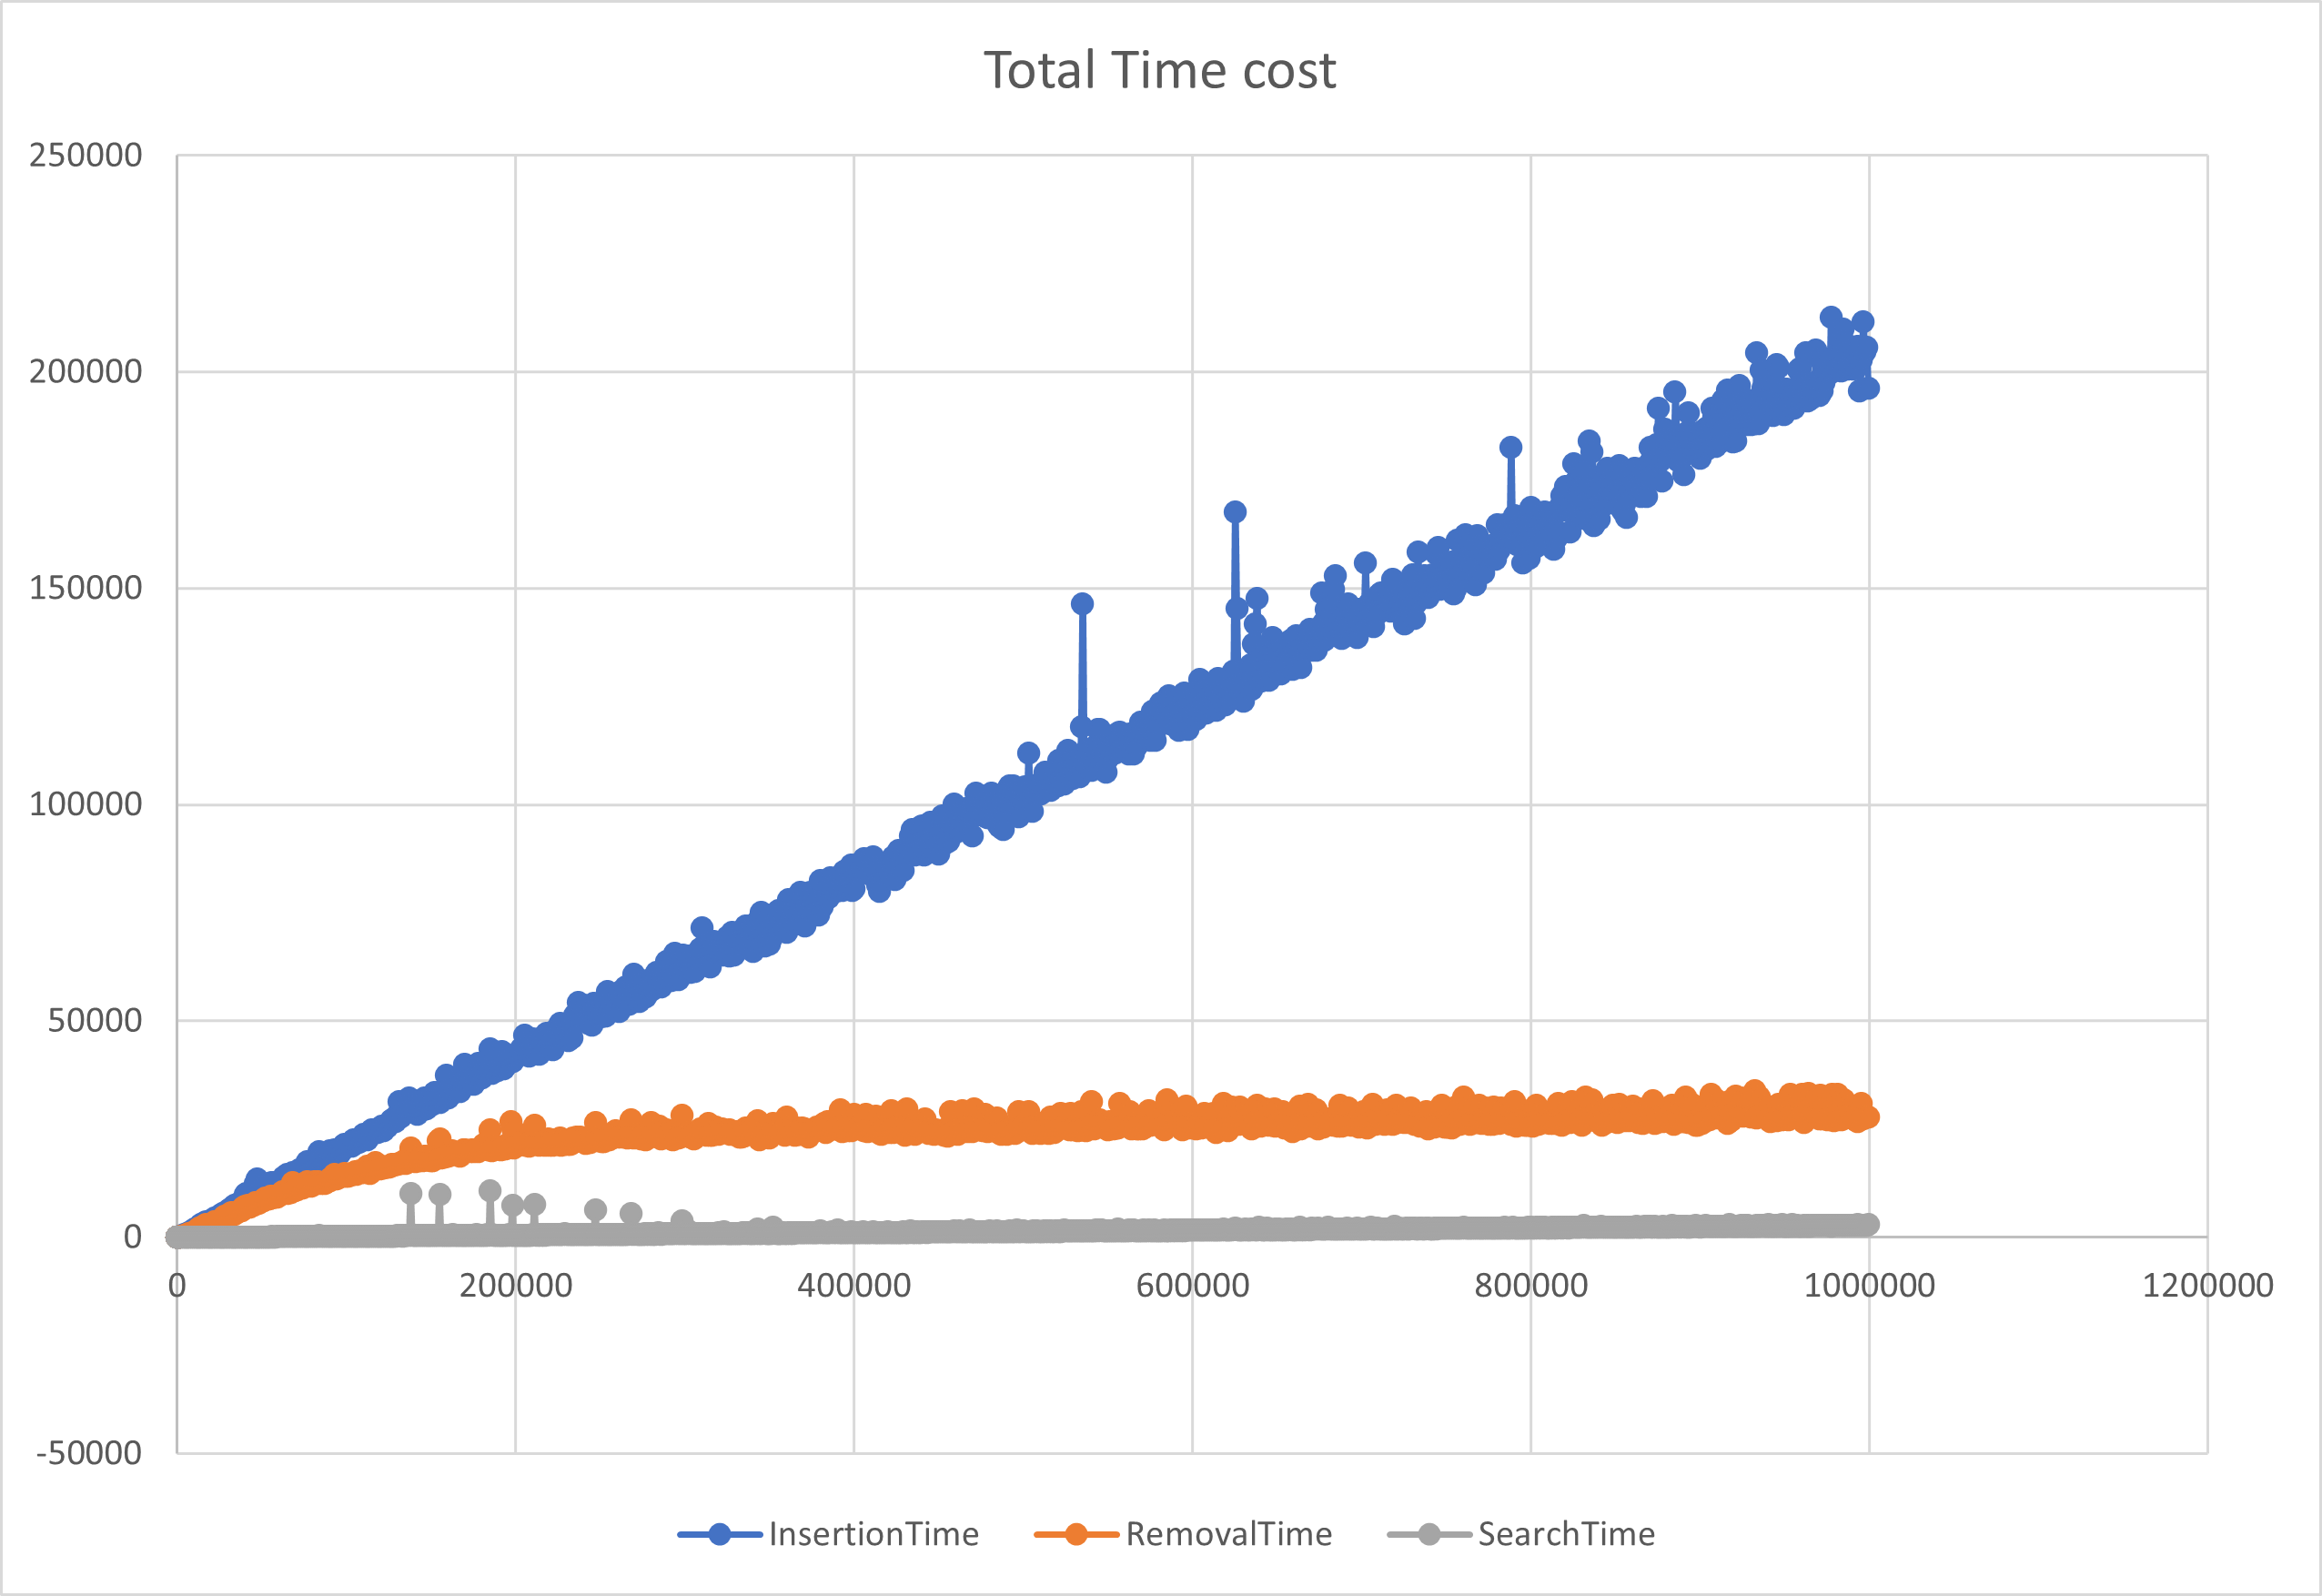
\includegraphics[width=0.5\textwidth]{pic0.png}
  \caption{Total cost of different operations}
  \label{average cost of different operations}
\end{figure}
Calculate the average cost of a single operation:
\begin{figure}[htbp]
  \centering
  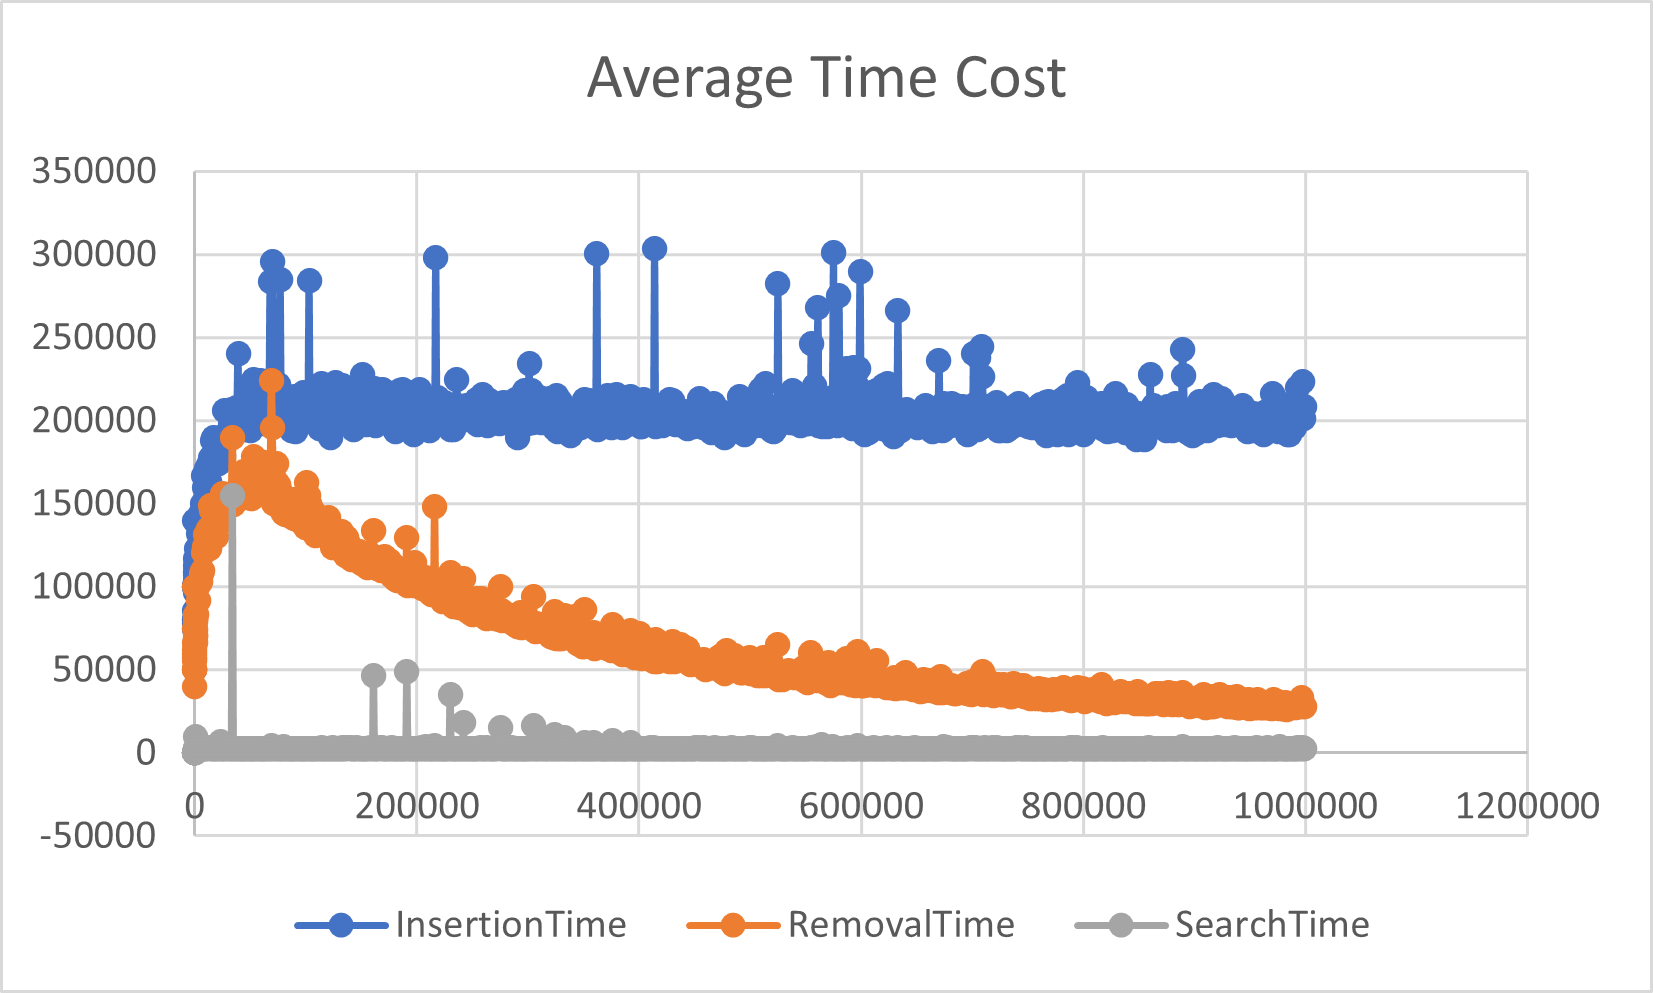
\includegraphics[width=0.5\textwidth]{pic1.png}
  \caption{average cost of different operations}
  \label{average cost of different operations}
\end{figure}

We can find that the time cost of this 3 operations are all $O(logn)$, sometimes even more faster than $logn$.

\section{Conclusion}
The Skip List is a powerful data structure that provides efficient support for insertion, deletion, and searching operations. By utilizing multiple levels and forward pointers, the Skip List achieves logarithmic time complexity for these operations.

In this experimental report, we have explored the principles behind the Skip List and compared its performance with a regular linked list. The Skip List offers significant advantages in terms of search efficiency and balanced height. It provides efficient insertion and deletion operations, making it a suitable choice for dynamic data structures.

However, it is important to consider the space overhead of the Skip List due to the additional forward pointers and multiple levels.

Overall, the Skip List is a versatile data structure that can be used in a wide range of applications where efficient search and update operations are required.

\end{document}
